% !Mode:: "TeX:UTF-8"
\chapter{相关概念阐述与理论基础}

\section{博物馆学习与导览概述}

\subsection{博物馆学习的界定与导览的情境化支持角色}
博物馆中的学习通常发生在真实参观过程中，观众会结合自身已有经验、兴趣动机和当下关注点来理解展品内容\cite{falk2016,li2024}。与目标明确、路径相对固定的学校教学相比，博物馆参观更接近一种开放式的探索活动。观众进入展厅后，会根据展陈内容、空间线索和个人兴趣自行选择停留对象与观看顺序，并在观看、比较、联想和提问中逐步形成理解\cite{falk2016}。因此，博物馆学习具有较强的开放性、自主性和过程性，其结果常常取决于观众在参观过程中如何与展品、环境和解释信息发生接触。

已有研究指出，博物馆体验会受到参观者原有知识基础、先前经验、参观目的和情感投入的持续影响\cite{falk2016,li2024}。面对同一件展品，不同观众的理解重点、兴趣深度和信息需求往往并不一致。有的观众希望快速建立对展区主题的整体认识，有的观众更关注某件具体文物背后的故事，也有观众会在参观过程中因为新的线索改变原本的兴趣方向\cite{falk2016}。这使得博物馆学习很难被看作一次统一、稳定的信息接收活动，它更像一个随着注意力转移和理解推进不断变化的认知过程。

在这一过程中，导览承担着重要的支持作用\cite{falk2016,li2024}。面对具有历史背景、文化语境和叙事关系的展品内容，观众往往很难仅凭展签文本或零散事实信息形成较完整的理解。很多时候，他们需要一个清晰的进入点，需要知道当前展品的重要性，需要理解它与前后内容之间的联系，也需要在信息量较大的环境中抓住真正值得关注的线索。导览能够在这一过程中提供帮助：它可以提示观看重点，补充必要背景，解释展品之间的关系，并通过适当的提问、追问或总结推动观众继续思考\cite{falk2016,li2024}。导览的价值因此落在“支持理解”上，而不只落在“补充信息”上。

从学习过程来看，观众对展品的理解通常是在不断接触和不断组织中推进的。最开始，某件展品可能只是因为造型、颜色、题材或展陈方式吸引注意；随后，观众会进一步产生“这是什么”“为什么重要”“和旁边那件有什么关系”之类的问题；在获得讲解、观察细节、阅读说明或与他人讨论后，理解才逐渐具体起来\cite{falk2016,li2024}。在这个过程中，导览能够帮助观众把分散的信息串联起来，使其从局部感兴趣转向对主题的进一步理解。对于部分内容密度较高、历史关联较复杂的展览，这种支持尤其重要，因为观众在缺少引导时很容易只记住零散知识点，难以形成较稳定的认识框架。

同时，博物馆导览还需要面对参观过程中的动态变化。观众的停留时间并不一致，注意力会波动，兴趣点会变化，理解深度也会随着参观推进不断调整\cite{falk2016}。有人在进入展区初期更需要简洁介绍，有人愿意在理解建立后继续追问细节，也有人会因为疲劳、时间限制或空间干扰而中断原本的观看节奏。在这种情况下，导览的作用不只是“把内容讲出来”，还包括在参观进程中持续提供合适的解释支持，帮助观众保持理解的连贯性。导览是否有效，很大程度上取决于它能否贴合观众在具体参观时刻的需求。

基于以上认识，本文将博物馆导览理解为一种嵌入参观过程的支持性活动\cite{falk2016,li2024}。它与观众的关注变化、理解状态和现场条件紧密相关，也会受到互动关系与环境因素的影响。为了进一步说明这些因素如何共同作用于博物馆学习，后文将引入情境学习框架，对个人、社会文化、物理环境及时间过程等维度展开讨论\cite{falk2016}。

\subsection{情境学习框架：个人、社会文化、物理及时间维度}
为理解博物馆学习在真实场景中的发生机制，Falk 与 Dierking 提出情境学习框架（Contextual Model of Learning），指出博物馆体验并不是由展品内容单独决定的，而是由参观者在参观过程中持续建构，其形成同时受到个人情境（personal context）、社会文化情境（sociocultural context）与物理情境（physical context）的共同影响，并需要在时间维度上进行整体把握\cite{falk2016}。这一框架强调，博物馆学习不是脱离环境与过程而独立发生的认知活动，而是在多重条件交织下展开的动态经验。

其中，个人情境主要涉及参观者带入博物馆的既有知识、兴趣动机、身份经验、先前记忆与注意取向等因素\cite{falk2016}。这些因素会影响参观者如何理解展览主题、对哪些对象产生兴趣、愿意在何处停留，以及如何生成问题与组织所获得的信息。即便面对同一展品，不同参观者也可能因为经验背景和目标差异而形成不同的理解路径\cite{falk2016,li2024}。因此，博物馆学习并不是对统一内容的标准化接受，而始终与个体的先在经验和即时状态密切相关。

社会文化情境强调学习并非完全私人化的认知过程，而是与互动关系、交流方式及文化解释框架密切相关\cite{falk2016}。在博物馆场景中，参观者可能通过与同伴的讨论、与讲解员的交流，或借助机构所提供的叙事结构与知识框架来组织理解。语言表达方式、互动角色关系以及沟通中的礼貌规范，也会影响参与意愿、提问方式和解释的接受度\cite{falk2016,luo2024}。这说明，博物馆中的理解过程并不只由“内容是否准确”决定，也与信息如何被表达、如何在互动中被共同建构密切相关。

物理情境则指向学习发生的空间与媒介条件，包括展厅环境、展品布局、观看距离、行进动线、标签文本以及数字媒介呈现方式等具体线索\cite{falk2016,luo2024}。这些要素会影响参观者最先注意到什么、能够停留多久、是否容易将局部信息联系为整体理解，以及是否能够在空间移动中保持认知连续性。换言之，博物馆学习并非只发生在头脑之中，也受到空间组织与媒介呈现方式的持续塑造\cite{falk2016}。

除上述三类情境外，时间维度贯穿于整个博物馆体验之中。Falk 与 Dierking 指出，个人、社会文化与物理情境并不是静止不变的，它们会随着参观推进不断变化并相互作用\cite{falk2016}。观众的兴趣强度、疲劳程度、理解深度、互动意愿及对后续内容的期待都会在时间中演化，这使得博物馆学习表现出明显的过程性特征。与此同时，该框架也提醒研究者，博物馆体验作为复杂系统只能被部分理解与部分控制，对不同情境因素进行区分更多是为了分析便利，而非意味着它们在真实参观中彼此孤立\cite{falk2016}。

\begin{figure}[htbp]
    \centering
    \includegraphics[width=\textwidth]{figure/figs/Contextual Model of Learning.png}
    \caption{Contextual Model of Learning 示意图（Falk 和 Dierking，2016）}
    \label{fig-contextual-model-learning}
\end{figure}

这一情境学习框架为理解博物馆导览提供了重要启发。它表明，导览不应被视为脱离具体参观条件的统一信息输出，而应被理解为嵌入个人状态、社会互动与空间环境之中的支持性活动。在博物馆参观具有非线性动线、兴趣驱动探索与理解逐步演化等特征的前提下，“情境”并不是导览发生的附属背景，而是理解导览如何发挥作用的重要前提。基于这一认识，后文将进一步讨论这些情境因素对于数字人导览设计的意义，以及它们如何影响导览过程中的交互组织与理解支持。

\section{对话式导览交互概述}

\subsection{对话式交互的关键特征：分层解释、追问延续与交互节奏}
在博物馆场景中，对话式导览的价值并不只在于回答观众提出的问题，还在于能否通过持续互动帮助观众逐步形成理解。已有研究表明，这类交互过程通常涉及三个彼此关联的方面：解释内容如何展开、问题如何在多轮对话中延续，以及互动如何在参与过程中保持合适的强度与节奏。结合相关研究，本文将对话式导览中的关键交互特征归纳为分层解释、追问延续与交互节奏三个方面。

（1）分层解释关注系统如何围绕同一对象组织不同层次的信息内容，使观众能够从较低理解门槛进入，再根据兴趣和需要逐步展开。其重点在于解释是否具有清晰的进入点、基本框架与后续延展空间，而不只是信息量的增减。在虚拟博物馆具身化对比实验中，拟人化导览员与“会说话的展品”在背景说明与细节补充上呈现出不同优势，说明解释层次可以通过不同角色与表达方式加以组织\cite{lopezgarcia2024}。相关导览研究也显示，用户持续期待“易于理解且确有帮助”的说明内容，这进一步表明，对话导览首先需要提供可进入的解释框架，再支持更具体的追问与补充\cite{hammady2021}。

（2）追问延续关注多轮对话能否围绕同一主题保持连续性，并在互动中逐步推进理解。对话导览的有效性并不体现在回答次数本身，而体现在回答之间是否能够形成语义递进、主题聚焦和探索积累，使观众从单点事实获取进一步走向关系理解和意义把握。相关研究表明，跨主题知识协同和互动历史利用能够提升多轮问答中的覆盖度与一致性，为持续追问提供支持\cite{varitimiadis2021}。在虚拟博物馆导航与推荐场景中，系统根据用户互动历史动态调整导览路线，同时用户对推荐依据表现出明确需求，这说明多轮导览不仅涉及问题回答，也涉及路径组织和反馈解释\cite{tsitseklis2023}。

（3）交互节奏关注系统如何通过回应长度、提示时机、提问方式与轮次安排来调节参与强度和认知负荷。博物馆导览并不是越频繁回应越有效，也不是信息越多越能促进理解。相关研究发现，封闭式问题与情境化提示能够提升用户的口头回应和现场互动质量，说明互动时机与表达方式会直接影响参与行为\cite{gasteiger2021}。同时，语言风格与具身化呈现也会影响停留时间、注视行为和情感投入\cite{noh2021}。这表明，对话导览中的节奏控制不仅是技术上的轮次安排，也关系到观众是否愿意继续参与、是否能够在当前强度下维持理解。

综上，现有研究提示，对话式导览的有效性主要体现在解释展开、问题延续和节奏调节三个方面。它们共同决定了导览交互能否从单次问答转向持续性的理解支持过程，也为后文进一步讨论对话式导览的设计要求提供了基础。

\subsection{对话式交互的优势与局限}
从交互方式来看，对话式导览的价值并不只体现在“能够回答问题”，还体现在它能够围绕用户输入持续组织解释、反馈与后续互动。首先，自然语言提供了较低门槛的信息入口，参观者可以直接围绕自身兴趣提出问题，无需依赖固定菜单或预设检索路径，从而降低信息获取过程中的操作负担。相关实地部署研究表明，这种交互方式有助于提升信息获取的便捷性与整体满意度\cite{duguleana2020}。对于参观者而言，对话导览的优势在于其更接近日常提问与交流习惯，能够让信息获取从“寻找功能”转向“围绕内容展开”。

其次，对话机制还能够增强导览过程中的主动参与感。与单向播报相比，对话式交互允许观众根据当下理解状态随时插入问题、请求补充说明或改变关注重点，这使导览过程更容易贴近个体化需求。相关研究表明，当对话机制与具身化呈现、历史重演式语言风格等设计结合时，用户的情感参与、认知价值感知以及停留和注视等行为指标都会受到影响\cite{noh2021}。此外，人设化聊天机器人研究也发现，语言风格与角色身份会影响用户对互动性、趣味性和记忆保持的感知\cite{sovic2025,suicmez2025}。MR 全息导览研究进一步指出，导览者角色会通过影响感知有用性与互动性，进而影响持续使用意图\cite{hammady2021}。这些结果共同说明，对话导览的优势不仅来自信息回答本身，也来自互动关系和参与方式的组织。

不过，对话式导览也存在明显局限。首先，多轮对话并不天然等于高质量导览。若系统缺少对当前对象、主题进展和用户状态的持续把握，对话过程就容易出现对象切换混乱、主题漂移或回应深度失衡等问题，使追问无法真正推动理解。相关研究提出“关键帮助（critical help）”策略，通过在互动过程中主动重构用户请求并与策展目标对齐来提升导览质量和个性化评价，这从侧面说明，对话交互要稳定发挥作用，还需要更明确的过程引导与目标约束\cite{cantucci2022}。

其次，生成式回答和个性化推荐虽然提升了交互流畅性，但也带来了可信度与可解释性问题。对于博物馆场景而言，观众通常不仅关心系统“说了什么”，也关心其依据何在、推荐从何而来。已有研究表明，用户对推荐缘由和证据线索存在持续需求，这意味着导览系统不能只提供表面上流畅的答案，还需要在必要时给出可核验的解释支持\cite{tsitseklis2023}。这一点在文化遗产和博物馆场景中尤为重要，因为相关内容往往涉及历史背景、文物属性和叙事关系，若缺少可靠依据，系统输出的价值会受到明显影响。

综合来看，对话式交互为博物馆导览提供了低门槛的信息入口、较强的参与弹性和持续推进理解的可能性，但它本身还不足以保证导览过程的稳定性与有效性。对话机制能够打开互动并推动交流，却仍需要与其他条件共同作用，才能支持更连贯、更可信的导览体验。基于这一认识，后文将进一步讨论在博物馆场景中，哪些因素会影响对话导览的持续性与有效性。

\section{具身数字人展示概述：导览中的多模态交互媒介}
\subsection{数字人作为导览媒介的交互价值}
在博物馆导览场景中，数字人除了呈现讲解内容，还承担导览媒介的组织功能。与展签、语音播报或菜单式检索等以信息输出为主的导览形式相比，具身数字人可以提供更明确的互动对象，使讲解过程围绕观众当下关注的展品、问题和理解状态展开。已有研究表明，具身化导览代理能够提升观众的参与感、临场感和参观完整度，使用户更愿意在虚拟展览中持续跟随导览过程，并减少对展品的遗漏\cite{garcia2024speaking,cao2021interactive}。这说明，数字人会直接影响观众如何进入互动、如何维持关注以及如何组织参观过程。如图\ref{fig-embodied-mediator}所示，数字人可作为导览代理连接对话交互、展品对象与观众理解，并通过提问、指向与引导等机制组织导览过程。

\begin{figure}[htbp]
    \centering
    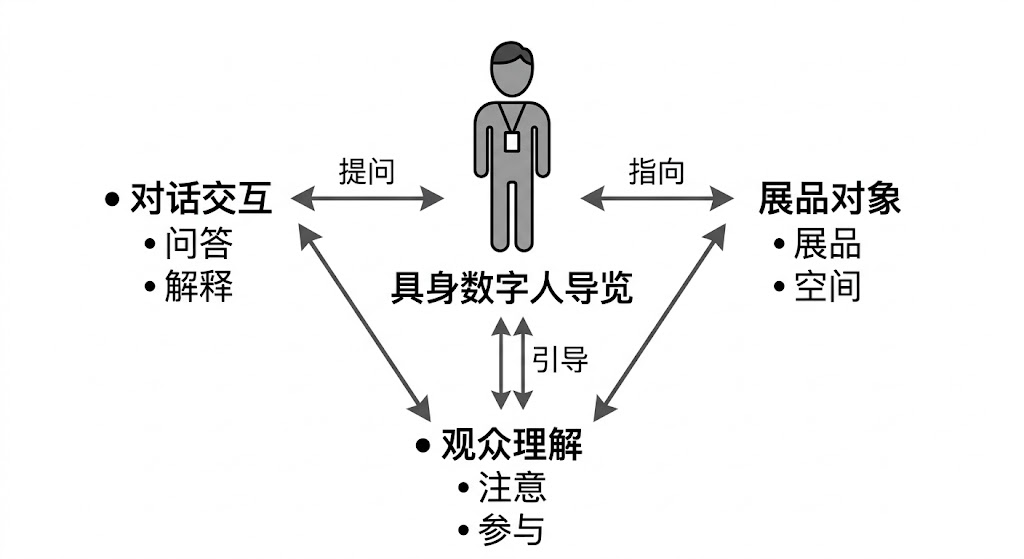
\includegraphics[width=\textwidth]{figure/figs/具身数字人在博物馆导览中的交互媒介结构.png}
    \caption{具身数字人在博物馆导览中的交互媒介结构。数字人作为导览代理连接对话交互、展品对象与观众理解，并通过提问、指向与引导等机制组织导览过程。}
    \label{fig-embodied-mediator}
\end{figure}

数字人作为导览媒介的另一项价值在于角色身份会影响观众参与导览的方式。观众在与数字人互动时，会同时判断讲解者身份、讲解风格和是否愿意继续跟随。当数字人以导览员、虚拟策展人、历史人物或具身化展品等角色出现时，其语言风格、开场方式和行为姿态都会改变观众对导览关系的理解。相关研究显示，个性化的初始互动设计能够显著提升用户对博物馆具身对话代理的信任与共情\cite{he2025icebreaking}；在虚拟博物馆场景中，不同具身形式也会影响观众的参与偏好与提问方式，具身化展品更容易引发细节追问与故事性交流\cite{garcia2024speaking}。这些结果表明，角色身份和开场互动会直接参与导览关系建立，并影响用户是否进入跟随导览的参观状态。

进一步来看，具身数字人能够增强导览过程中的临场感，使对话关系更容易被感知和维持。与缺少视觉承载的问答系统相比，数字人通过可见角色形象、连续表达方式以及与空间对象相关联的行为线索，使互动过程更容易被观众理解为持续发生的交流过程。相关研究表明，在博物馆与虚拟展览场景中，具身化代理能够提升用户对互动性、趣味性和记忆保持的主观感知，同时改善整体参观体验与信息可达性\cite{duguleana2020va,cao2021interactive}。这为后续解释展开、提问延续和参与维持提供了较稳定的交互基础。

\subsection{多模态表达对注意力组织与理解支持的作用}
在博物馆导览中，观众理解效果既取决于系统讲解内容，也取决于内容呈现方式。数字人的视线、手势、身体朝向、语气和停顿等多模态表达，会直接参与解释组织，并影响观众如何分配注意力、识别重点以及将语言内容与现场对象联系起来。对于展品密集、信息层次复杂的场景，单靠语言说明往往难以保证观众始终跟上讲解进程；多模态表达能够补充感知线索，使解释过程更具可进入性和层次感。相关研究表明，共语手势能够显著提升具身对话代理在人型感、活力感和感知智能等方面的评价，并吸引和维持用户视觉注意\cite{pereira2022cogesture}。这说明，多模态行为是解释展开的重要交互资源。

多模态线索还可以帮助观众将语言说明与具体展品对象、空间位置和观看行为对齐。博物馆导览通常发生在包含多个展品、空间动线和环境线索的复杂场景中，观众需要不断判断当前讲解对应哪件展品、哪一处细节以及接下来应当关注哪里。此时，视线方向、指向动作和身体朝向等表达能够提供明确的对象定位线索，使观众更容易把听到的内容与看到的对象对应起来。虚拟博物馆研究也表明，不同具身形式会引导用户产生不同类型的关注与提问：拟人化导览员更适合承载整体背景说明，具身化展品更容易引发围绕自身故事与细节的追问\cite{garcia2024speaking}。这说明，具身表达会影响互动围绕什么对象展开，并参与导览中的对象组织和理解支持。

多模态表达还参与追问延续与交互节奏组织。前文指出，对话式导览能否有效推进，取决于多轮互动中主题连续性、解释递进性和节奏适配性。人类面对面对话研究进一步表明，轮转接续具有多模态特征：视线方向和手势完成情况会影响说话轮次衔接，带有手势的轮转通常转接更快，也更有助于参与者协调发言时机\cite{kendrick2023turntaking}。这为具身数字人导览提供了启发：在导览场景中，稳定的面向对象状态、与当前主题一致的动作语气，以及适度停顿和提示，都有助于观众判断互动是否仍在同一讲解脉络中展开，并降低多轮互动中的跳跃感和断裂感。整体来看，多模态表达参与了注意力组织、轮次协调和理解支持。

\subsection{具身展示在导览体验整合中的意义}
从整体角度看，具身数字人的价值体现在把讲解内容、空间环境与观看过程组织为较连贯的导览体验。博物馆参观是持续变化的信息接触过程，观众始终处在移动、停留、观察、比较和判断之中，讲解内容需要不断与这种观看过程发生联系。具身数字人为这一联系提供了更明确的组织方式：它可以承载讲解内容，也可以通过角色身份、行为提示和空间指向参与导览引导，使导览活动更容易嵌入真实参观情境。相关研究表明，交互式具身代理能够提升临场感，也能提升虚拟展览中的参观完整度，体现出沉浸价值以及路径引导和任务完成价值\cite{cao2021interactive}。这意味着，数字人可以作为连接内容、空间与行动的导览中介。

这种整合作用还体现在数字人能够帮助组织用户探索路径与叙事层次。虚拟博物馆的具身化研究指出，人形导览员与具身化展品可以承担不同导览职能：前者更适合整体背景引入与情境说明，后者更适合围绕具体对象展开细节叙述和故事性互动\cite{garcia2024speaking}。这说明，具身展示可以在导览过程中承担不同层次组织功能，帮助用户在整体理解与局部深入之间建立更清楚的路径。此外，面向虚拟展览的相关平台研究也显示，当叙事结构、空间浏览和个性化导览建议整合在同一系统中时，用户更容易形成连贯参观体验，并在探索过程中保持对展览主题的理解连续性\cite{zidianakis2021invisible}。这些结果共同表明，具身代理有助于观众在空间和叙事层面建立更稳定的跟随关系。

因此，在博物馆导览场景中，具身展示提升了用户兴趣，也提升了导览过程的可跟随性与连续性。3.1 强调导览是情境化理解支持，这一判断在数字人交互中获得了更具体形态；3.2 归纳的解释展开、追问延续与交互节奏，也可以通过具身表达转化为更可感知的导览过程。数字人会影响导览如何被感知、如何被跟随以及如何在空间中持续展开。基于这一点，后文将进一步讨论对话组织、情境因素与具身表达之间的协同关系，并在此基础上展开后续设计框架分析。

\section{本章小结}
本章围绕博物馆学习、对话式交互与具身数字人展示三个方面，对本文研究涉及的相关概念与理论基础进行了梳理。首先，博物馆学习发生在参观过程中，个人状态、社会互动、空间环境及时间推进会共同影响意义建构。由此，导览的价值体现在传递展品信息与提供理解支持两个层面，重点在于将支持机制嵌入参观过程。其次，对话式导览相较于菜单式检索或固定脚本讲解，能够以更低门槛支持提问、解释展开与持续互动，并在分层解释、追问延续和交互节奏等方面展现出导览推进潜力；其有效性仍会受到主题连续性、过程组织与解释可信性的限制。最后，具身数字人作为对话交互的可感知媒介，视线、手势、朝向、语气和停顿等多模态表达会参与注意力组织、对象对齐和互动维持，并进一步影响导览过程的感知与跟随。

综合来看，博物馆导览中的数字人交互涉及内容组织、情境把握与具身表达三个层面的协同，是一个复合设计问题。前文理论梳理表明，若要使数字人导览从“能回答”走向“能引导”，需要将对话推进、参观过程中的情境支持以及可感知的具身表达放在同一分析视角下讨论。
